%!TEX root = root.tex

%% Dans cette section, nous faisons un retour d'expérience sur l'usage
%% d'{\Asak} pour la détection de clones dans les paquets~\Opam. Nous
%% commençons par détailler notre approche puis quelques résultats
%% préliminaires.

%% La redondance de code est un des fléaux de l'informatique moderne. Elle entraine inévitablement une grande difficulté de maintien (si l'on change une définition, il faudrait changer tous ses clones), de compréhension (nous ne dénombrons pas moins de 30 noms différents pour la célèbre fonction \iocaml{Option.map} dans la moitié des paquets \Opam) et des pertes de temps énorme consacrés à redéfinir des fonctions usuelles (nous dénombrons quelques 142 implémentations de ~\iocaml{Option.map}  dans la moitié des paquets \Opam).

\paragraph{Approche utilisée}

Contrairement à l'environnement bien contrôlé des
copies~{\LearnOCaml}, chaque paquet~{\Opam} a un ensemble de
dépendances et une logique de compilation potentiellement complexe.
Pour ces paquets, la phase d'extraction des termes {\LambdaCode}
nécessite donc une configuration spécifique de la partie avant du
compilateur. Il serait difficile d'automatiser cette configuration à
partir du contenu des paquets. Nous avons préféré créer une version
personnalisée du compilateur~{\OCaml}~\cite{custom-ocaml} installable
dans \textit{switch} {\Opam}.
%
Le compilateur modifié instrumente la compilation standard par un
mécanisme de normalisation et d'exportation des termes~{\LambdaCode}.
Le dossier contenant le fichier source permet au compilateur de connaître le
paquet~{\Opam} en cours d'installation. Chaque terme collecté peut
ainsi être étiqueté par le nom du paquet~\Opam, par le nom du fichier
source et par le chemin du module de la définition dont il est issu.

À l'aide d'un serveur de calcul~\footnote{Une machine possédant 40
processeurs Intel(R) Xeon(R) CPU E5-4640 v2 cadencé à 2.20GHz équipé
de 756Go de RAM.}, nous avons ensuite parallélisé les (tentatives
d')installations de l'ensemble des paquets~\Opam. Au bout de~$20$
heures, nous avons obtenu un corpus de travail dont nous rapportons
maintenant l'analyse avec~{\Asak}.

\paragraph{Portée de l'analyse}

Nous avons réussi à compiler $1250$ paquets sur les $2428$ paquets que
compte à ce jour le dépôt {\Opam} officiel. Tous les paquets n'ont pas
pu être installés car
certains paquets ne compilent pas avec {\OCaml} 4.08.1 ou
sont en conflit avec {\OCaml} 4.08.1 ; ou bien encore parce que
certains paquets dépendent de bibliothèques C non-installées.

\paragraph{Aspects quantitatifs}

Sur ces $1250$ paquets, nous avons extrait $360152$ définitions
strictement différentes. On a retiré de ce décompte les définitions
provenant de deux versions différentes d'un même paquet et qui
produisent la même empreinte.

En ne conservant que les empreintes des sous-arbres de plus de~$30$
nœuds (limite calculable en temps raisonnable de notre
implémentation), ces définitions ont été classées en $198841$ classes,
dont $40935$ avec strictement plus d'un élément (c'est-à-dire que nous
avons identifié au moins $40935$ doublons). Le tout a été calculé en
$40$ minutes sur la machine décrite précédemment. Voici un diagramme à
barre synthétisant la forme des classes obtenues (attention,
l'échelle des ordonnées est logarithmique).

\begin{figure}[h]
\begin{center}
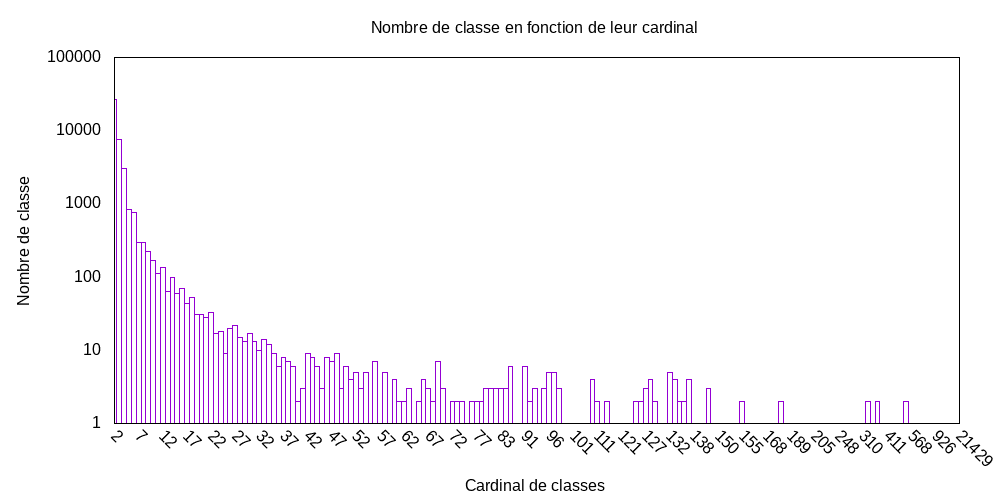
\includegraphics[width=10cm]{figures/bars.png}
\end{center}
\end{figure}

\paragraph{Aspects qualitatifs}

Les classes comprenant plus de 50 éléments sont majoritairement de
deux types. Il s'agit d'une part de très petites fonctions (des
variables globales ou des fonctions constantes). Comme {\Asak} ne
prend pas en compte la valeur des littéraux, ces dernières sont toutes
regroupées. L'autre type de redondance est issu du code généré par des
outils comme \verb|Coq|, \verb|Menhir|, \verb|AWS|...
\yrg{Quand tu parles de code généré par AWS, je ne suis pas sûr de voir de quoi tu parles.}

Cependant, certaines classes représentent de véritables possibilités
de factorisation. Par exemple, nous trouvons une classe contenant
$122$ éléments comprenant toutes les définitions de la (célèbre)
fonction \iocaml{Option.map}, que l'on trouve sous pas moins de $32$
noms différents. Cette classe capture aussi les fonctions similaires
concernant les types isomorphes au type \iocaml{option}. Par exemple,
cette classe contient la fonction \iocaml{map_evar_body} (provenant du
module \iocaml{Evd} de \verb|Coq|):

\begin{ocaml}
let map_evar_body f = function Evar_empty -> Evar_empty | Evar_defined d -> Evar_defined (f d)
\end{ocaml}

Une synthèse complète de l'analyse des paquets~{\Opam} par~{\Asak} sera l'objet
de travaux futurs.
